\section{Experiments}
\label{sec:experiments}

\begin{figure*}[t]
    \centering
    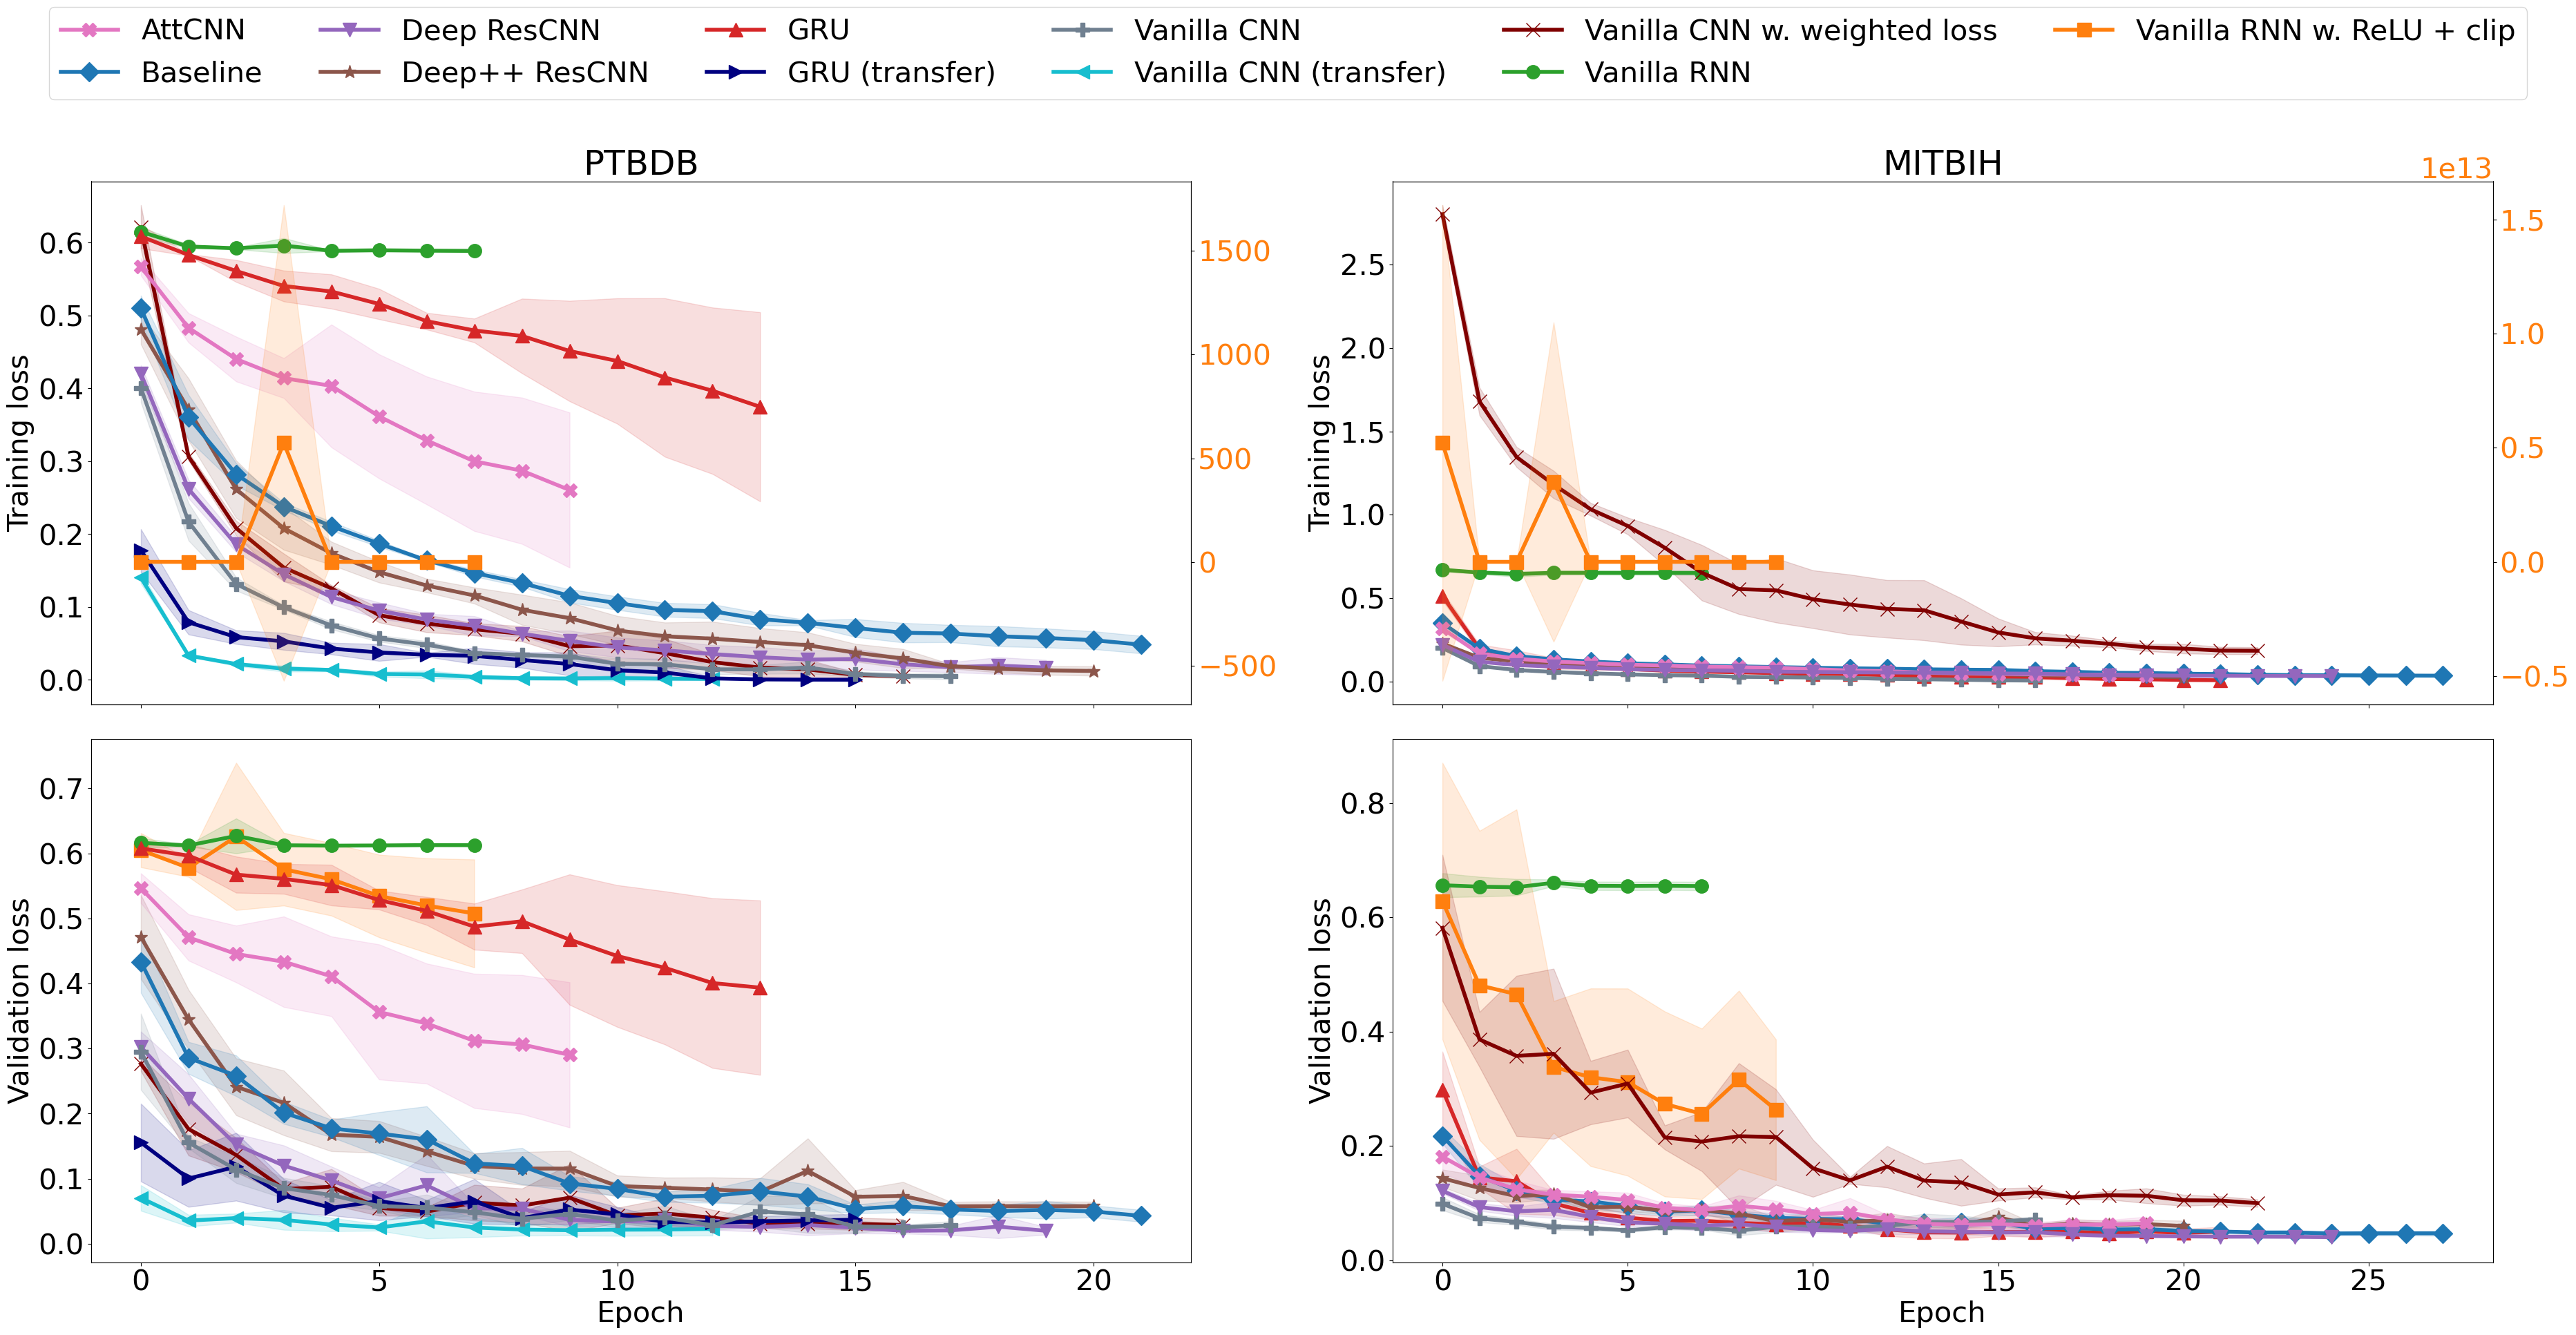
\includegraphics[width=0.70\textwidth]{figures/learning_curves.png}
    \caption{Learning curves for our deep-learning models showing the mean (upper) training and (lower) validation cross-entropy loss by epoch on the (left) PTB DB and (right) MIT-BIH datasets. The shaded areas depict \boldmath$\pm 1$ standard deviation from the mean. The second \boldmath$y$-axes (rhs) depicts the training loss for the Vanilla RNN w. ReLU + clip model.}
    \label{fig:learning_curves}
\end{figure*}

\subsection{Experimental Setup}
All of our experiments were performed on the ETH Euler cluster\footnote{\url{https://scicomp.ethz.ch/wiki/Euler}} using 1 unknown GPU and 1 unknown CPU with 8 GB of reserved RAM. We repeated every model run five times with consecutive seeds (seed 42 to 46) and report the mean and standard deviation. The tree-based models were developed using Scikit-learn \citep{scikit-learn}. The deep-learning models were developed using Tensorflow \citep{tensorflow2015-whitepaper} and were trained for a maximum of 1000 epochs using the Adam optimizer \citep{kingma2014adam} and decreasing the learning rate once validation accuracy plateaued for 3 epochs. We further used early stopping and assumed convergence when the validation accuracy showed no improvement for 7 (5 for baselines) consecutive epochs. The final models are the models with the highest validation accuracy.

Hyperparameter tuning was done using a random search \citep{bergstra2012random} over a large parameter space for both model and optimizer configurations. Optimal configurations can be found in the source code. We further experimented with Bayesian optimization to tune some models but this showed no improvement over a vast random search. It had a slightly higher compute efficiency but increased implementation complexity significantly.

For the MIT-BIH dataset, the F1-score is computed as the macro-averaged or unweighted mean of all per-class F1-scores. For the PTB DB dataset, we use AUPRC to denote the average precision score since directly computing the area under the precision-recall curve using the trapezoidal rule is prone to overestimating\footnote{See \url{https://scikit-learn.org/stable/modules/generated/sklearn.metrics.average_precision_score.html}.}



\subsection{Results and Discussion}

\subsubsection{Training behavior}
The training behavior of all deep-learning models models is shown in \autoref{fig:learning_curves}. As expected, larger models train slightly slower. They also exhibit greater variance in loss and final accuracy depending on the seeding. For the \textsc{VanillaRNN} model with Tanh activation and no gradient clipping, we find that it suffers from the vanishing gradient problem causing stagnating loss. \textsc{VanillaRNN+ReLU+Clip} performs much better, however, we observe divergence of loss, presumably due to large gradients, temporarily for some runs.

\begin{figure*}[t]
    \centering
    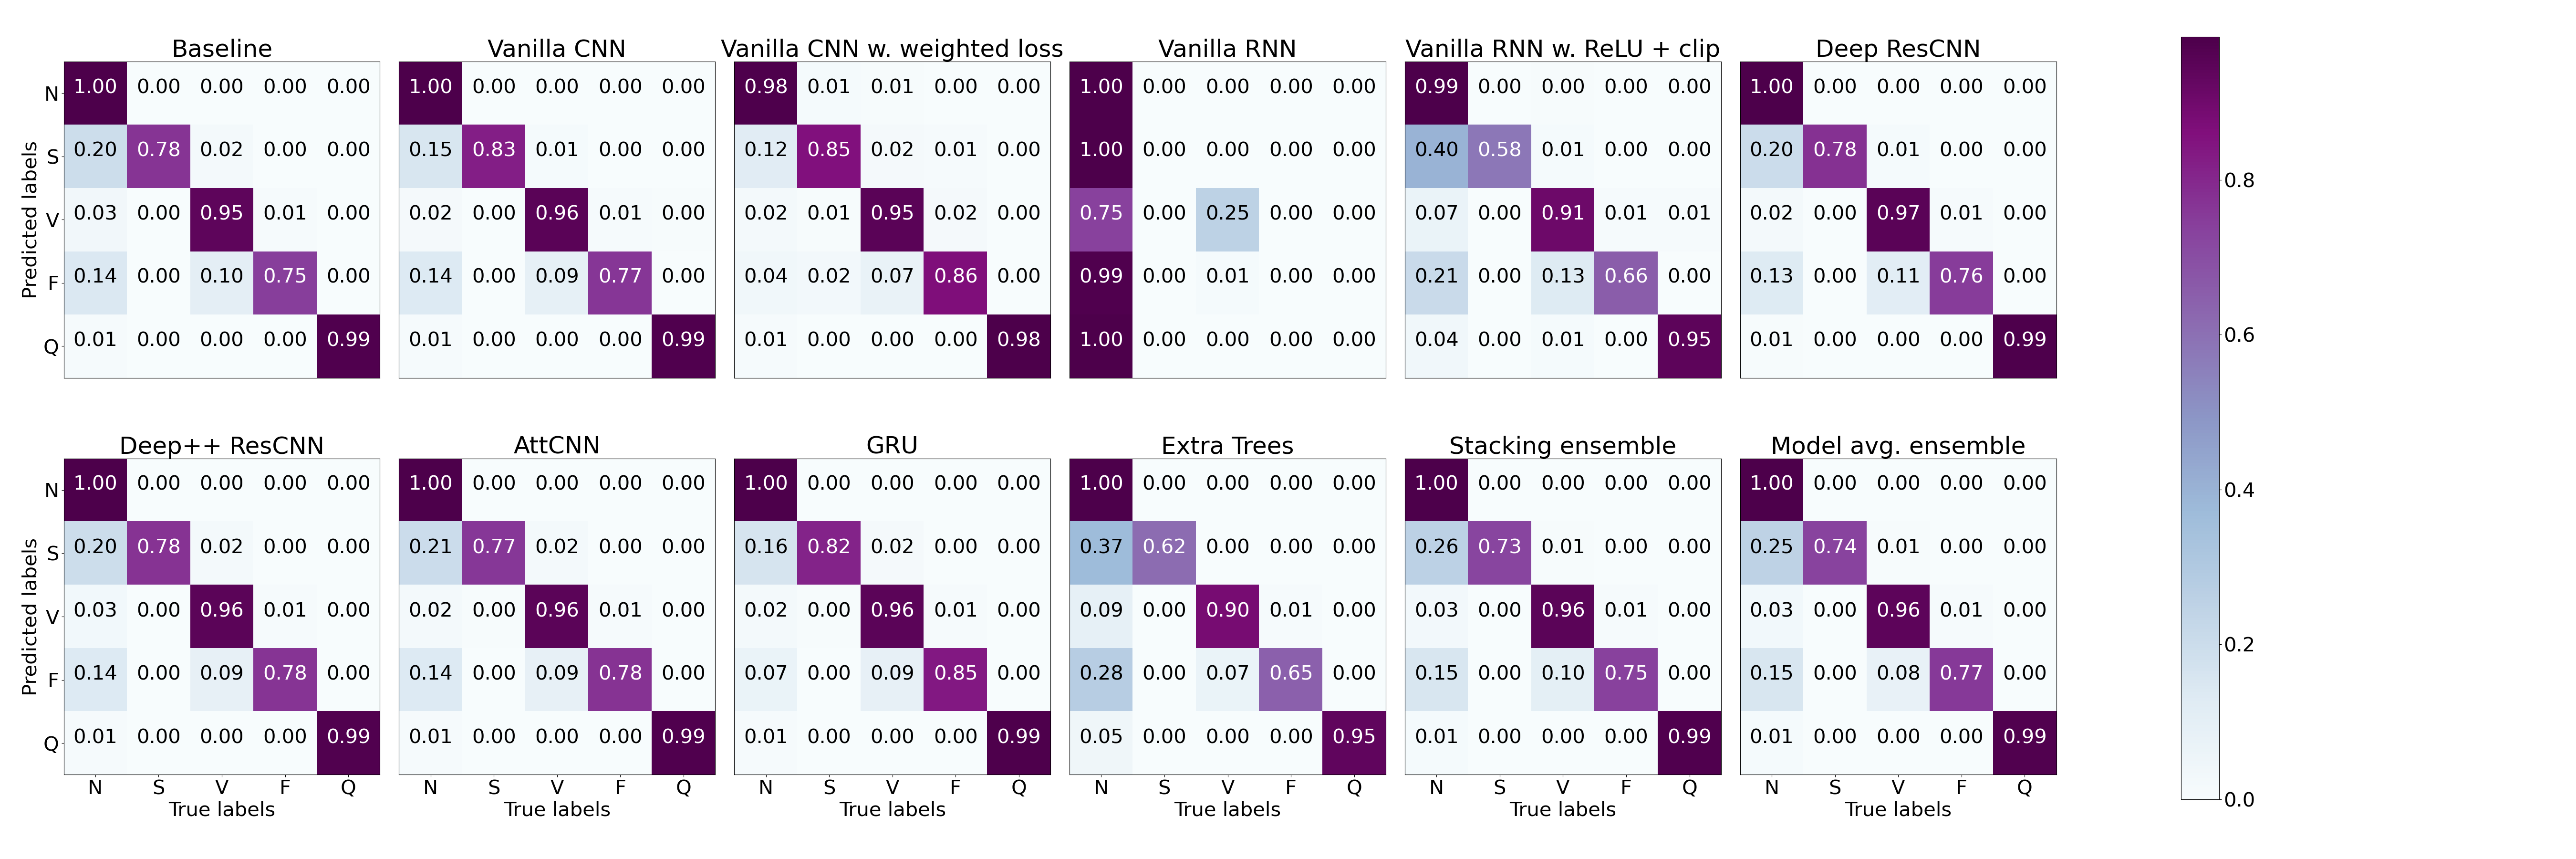
\includegraphics[width=1\textwidth]{figures/confusion_matrices_mitbih.png}
    \caption{Confusion matrices associated with our model performances on the MIT-BIH test dataset. The class abbreviations are as follows: 'N' is normal beat, 'S' is supraventricular premature beat, 'V' is premature ventricular contraction, 'F' is fusion of ventricular and normal beat, and 'Q' is unclassifiable beat.}
    \label{fig:confusion_matrices_mitbih}
\end{figure*}

\begin{figure}[]
    \centering
    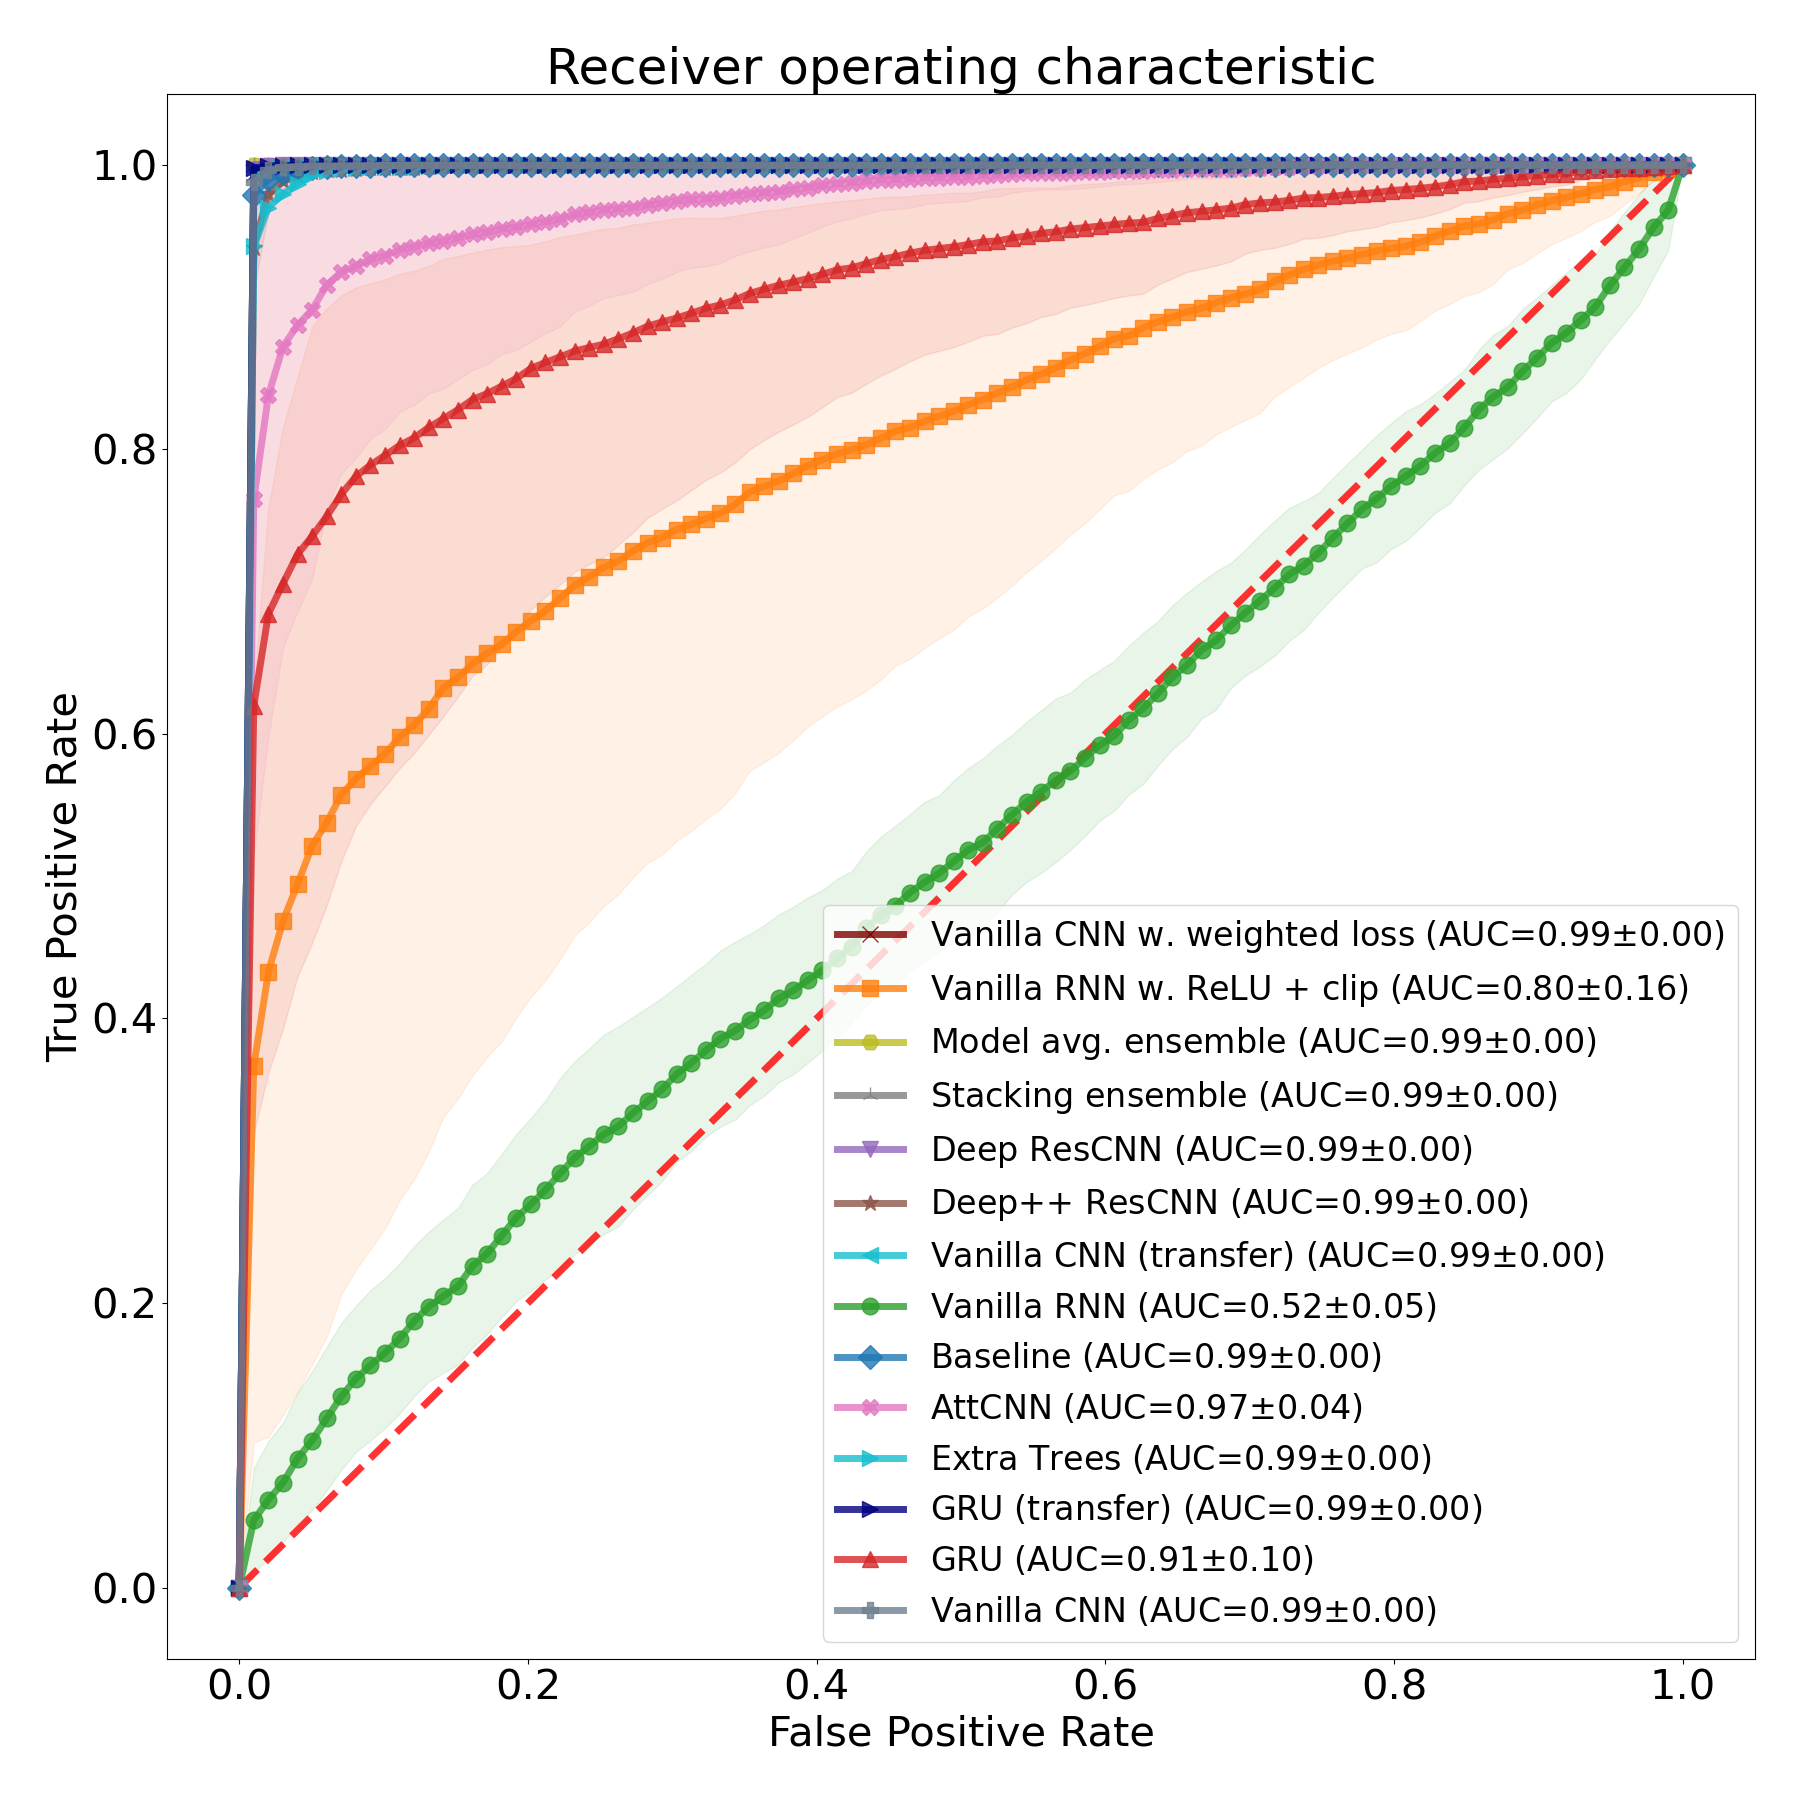
\includegraphics[width=0.3\textwidth]{figures/roc_ptbdb.png}
    \caption{Receiver operating characteristic curve for our models on the PTB DB test dataset. The shaded areas depict \boldmath$\pm 1$ standard deviation from the mean.}
    \label{fig:roc_ptbdb}
\end{figure}

\subsubsection{Test scores}
\autoref{tab:results_ptbdb} and \autoref{tab:results_mitbih} show the performance metrics on the test sets. Generally, we observe good performance close to the baseline for most models. Notably our \textsc{VanillaCNN} shows good performance, outperforming the baseline on both datasets. However, adding model complexity does not yield better results as evident by the performance of \textsc{Deep++ ResCNN} and \textsc{AttCNN}.

In line with the observed stagnating loss, \textsc{VanillaRNN} with Tanh activation and no gradient clipping fails to produce useful outputs for both datasets. As seen in the confusion matrix in \autoref{fig:confusion_matrices_mitbih} as well as the ROC curve in \autoref{fig:roc_ptbdb}, it is clear that it does not perform better than random chance. The RNN-based models, \textsc{VanillaRNN+ReLU+Clip} and \textsc{GRU}, perform much better, especially on the MIT-BIH dataset. On the smaller PTB DB dataset they lack performance. This can likely be explained by the fact that they require more training data due to a large amount of parameters. This may also help explain why \textsc{GRU} benefits greatly from transfer learning, outperforming all other non-ensemble models on PTB DB. The smaller \textsc{VanillaCNN} does not benefit as much from transfer learning, showing only a small improvement.

The tree-based models, \textsc{Extra Trees}, produce predictions that are useful, yet not competitive with the baseline. They, however, train much faster than the deep learning models leading to a trade-off between performance and training time.

As seen in \autoref{fig:confusion_matrices_mitbih}, a weighted loss may balance class frequency effects as shown by the improved performance for \textsc{VanillaCNN} in predicting minority classes after being trained with the weighted loss. Overall accuracy and F1 score does decrease as another trade-off. We note that this behavior may be desired in some settings where, e.g., false negatives are more problematic for specific classes such as in medical domains.

Finally, as expected, the ensemble methods building upon all models and their variations perform very well. Both of their accuracies are within around a standard deviation of the best performing model on both datasets, outperforming all other models at times. Still, \autoref{fig:confusion_matrices_mitbih} shows that the ensemble methods inherit the minority class inaccuracies of the models that they build upon.
